\documentclass[11pt,a4paper]{article}

%-------------------Packages-------------------%
\input Acorn.fd
\usepackage[magyar]{babel}
\usepackage[T1]{fontenc}
\usepackage{kpfonts}
\usepackage{changepage}
\usepackage{xcolor}
\usepackage{tikz}
\usepackage{wrapfig}
\usepackage{hyperref}
\usepackage{fancyhdr}
\pagestyle{fancy}
\usepackage{anyfontsize,lettrine}

%-------------------Settings-------------------%
\graphicspath{{./images/}}
\setlength\parindent{0pt}


\cfoot{}

\lhead{\rightmark}
\rhead{\thepage}
\setcounter{DefaultLines}{3}
\renewcommand{\LettrineFontHook}{\usefont{U}{Acorn}{xl}{n}}
%-------------------Commands-------------------%
\newcommand{\AUTHOR}{Herőczi Sándor}
\newcommand{\NEPTUN}{WH0AMC}
\newcommand{\TITLE}{Automata fegyverrendszer tervezése}
\newcommand{\YEAR}{2024}
\newcommand{\LOCATION}{Budapest}

%-------------------Colours-------------------%
\definecolor{BMEbordo}{HTML}{862633}


\begin{document}

\begin{titlepage}
	\begin{adjustwidth}{-2.5cm}{-2.5cm}

	
	\thispagestyle{empty}
	\centering

	\LARGE
	\rule{16cm}{1pt}\\
	\textsc{
		Budapesti Műszaki és Gazdaságtudományi Egyetem\\
		Villamosmérnöki és Informatikai Kar\\
		Automatizálási és Alkalmazott Informatikai Tanszék}\\[-0.3cm]
	\rule{16cm}{1pt}
	\end{adjustwidth}
	
	\vspace{2cm}
	
	\flushleft
	\Huge
	\textcolor{BMEbordo}{\textbf{\TITLE}}
	
	\vspace{3cm}
	
	\Large
	\textbf{\AUTHOR}\\
	\NEPTUN\\
	
	\begin{tikzpicture}[overlay, remember picture]
		\node[anchor=center, xshift=5cm, yshift=-10cm] at (current page.center)
		{\includegraphics[height=2cm]{autlogo}}; 
	\end{tikzpicture}
\end{titlepage}

\section{Bevezetés}

\subsection{Az automata fegyverrendszerekről}

\lettrine{M}{int} manapság az ipar minden területén, így a fegyveriparban is egyre nagyobb mértékű a digitalizáció és az automatizáció. Ennek ékes példája a távolról irányítható lőállások térnyerése, amelyeknek nagy előnye a fegyver és a tüzér egymástól való elkülönítése, aminek több előnye is van. Természetesen a legfontosabb és leginkább szembetűnő, hogy ezzel a módszerrel minimalizálható, vagy akár megszüntethető a saját embereink életének kockáztatása. Ezentúl olyan helyen is tudjuk használni ezeket az eszközöket, ahova egy tradicionális géppuskafészek telepítése nehézkes lenne, például mostoha természeti körülmények közé, egy torony tetejére, vagy akár egy hadihajó oldalára. Szintén egy nagy előny, hogy ezek az eszközök felszerelhetők több kezeléssegítő alegységgel, például hőkamerával vagy éjjellátóval. Majdnem minden, számottevő hadsereggel rendelkező országnak van saját fejlesztésű távirányított fegyverrendszere.\\


\begin{wrapfigure}{r}{0.45\textwidth}
	\centering
	\includegraphics[width=0.9\linewidth]{irod_phalanx} 
	\caption{Phalanx CIWS rendszer}
	\label{fig:irod_phalanx}
\end{wrapfigure}

A következő lépés az automatizálás. Hiszen egyre erősebb hardverekkel rendelkezünk, egyre jobb algoritmusokat tudunk implementálni, és elértük az a szintet, hogy bizonyos helyzetekben a "gép" jobb munkát tud végezni, mint egy ember. Az első automatikus célzórendszerrel rendelkező légvédelmi gépágyú az amerikai \textsl{Phalanx CIWS} az 1970-es években került kifejlesztésre, ezzel megszületett a "Lethal autonomous weapon (LAW)" kifejezés.\\

A technológiát érthető módon leggyakrabban védelmi célokra használják, sokszor légvédelemre. A gyakorlatban nagy szerepe van Dél-Korea és Izrael védelmében, ahol a rakétatámadások mindennapos veszélyt jelentenek. Offenzív célokra a gyakorlatban még csak rakéták célzására használnak automatikát, a "terminátor" jellegű gyilkos robotok még csak fejlesztési fázisban vannak.\\


\pagebreak
\subsection{Irodalomkutatás}
A legjelentősebb katonai hatalmak mindegyike rendelkezik távvezérelt fegyverrendszerekkel, leggyakrabban valamilyen távolról irányított gépfegyver formájában. Azonban se az egyes országok nemzetbiztonságának, se a fegyveripari partnercégeknek nem áll érdekében a szükségesnél több információt kiadni. Ez egy kicsit megnehezítette az irodalomkutatást, de a képek alapján azért sok információt ki lehet nyerni.\\

\subsection{Elrendezés}

Az egyik legnagyobb darabszámban gyártott távirányított fegyverrendszer az amerikai \textsl{CROWS} rendszer, amely a NATO-országokban, köztük Magyarországon is rendszeresített HMMWV páncélozott járművekre telepíthető. Több verziója létezik több kaliberrel, a \ref{fig:irod_crows}. ábrán egy M240B géppuskával látható.

\begin{figure}[h!]
	\centering
	\includegraphics[width=1\linewidth]{irod_crows}
	\caption{Az amerikai CROWS rendszer}
	\label{fig:irod_crows}
\end{figure}

Az ábrán megfigyelhető, hogy a fegyver csöve nagyjából egybeesik a függőleges és vízszintes mozgástengelyekkel. Szintén jól látható a fegyverrel együtt mozgó kamera kialakítása is.\\

A \textsl{CROWS} rendszer orosz megfelelője a hasonló kialakítású \textsl{Arbalet-DM} (\ref{fig:irod_arbalet}.ábra). Ennek a rendszernek az alapja a 12.7 mm-es KORD nehézgéppuska. Rendelkezik 4 gránátvetővel is, amelyek füstfüggöny felhúzására használható. A kamera és a fegyver elhelyezése, de még a lőszer pozíciója is teljesen hasonló az amerikai párjához.

\begin{figure}[h!]
	\centering
	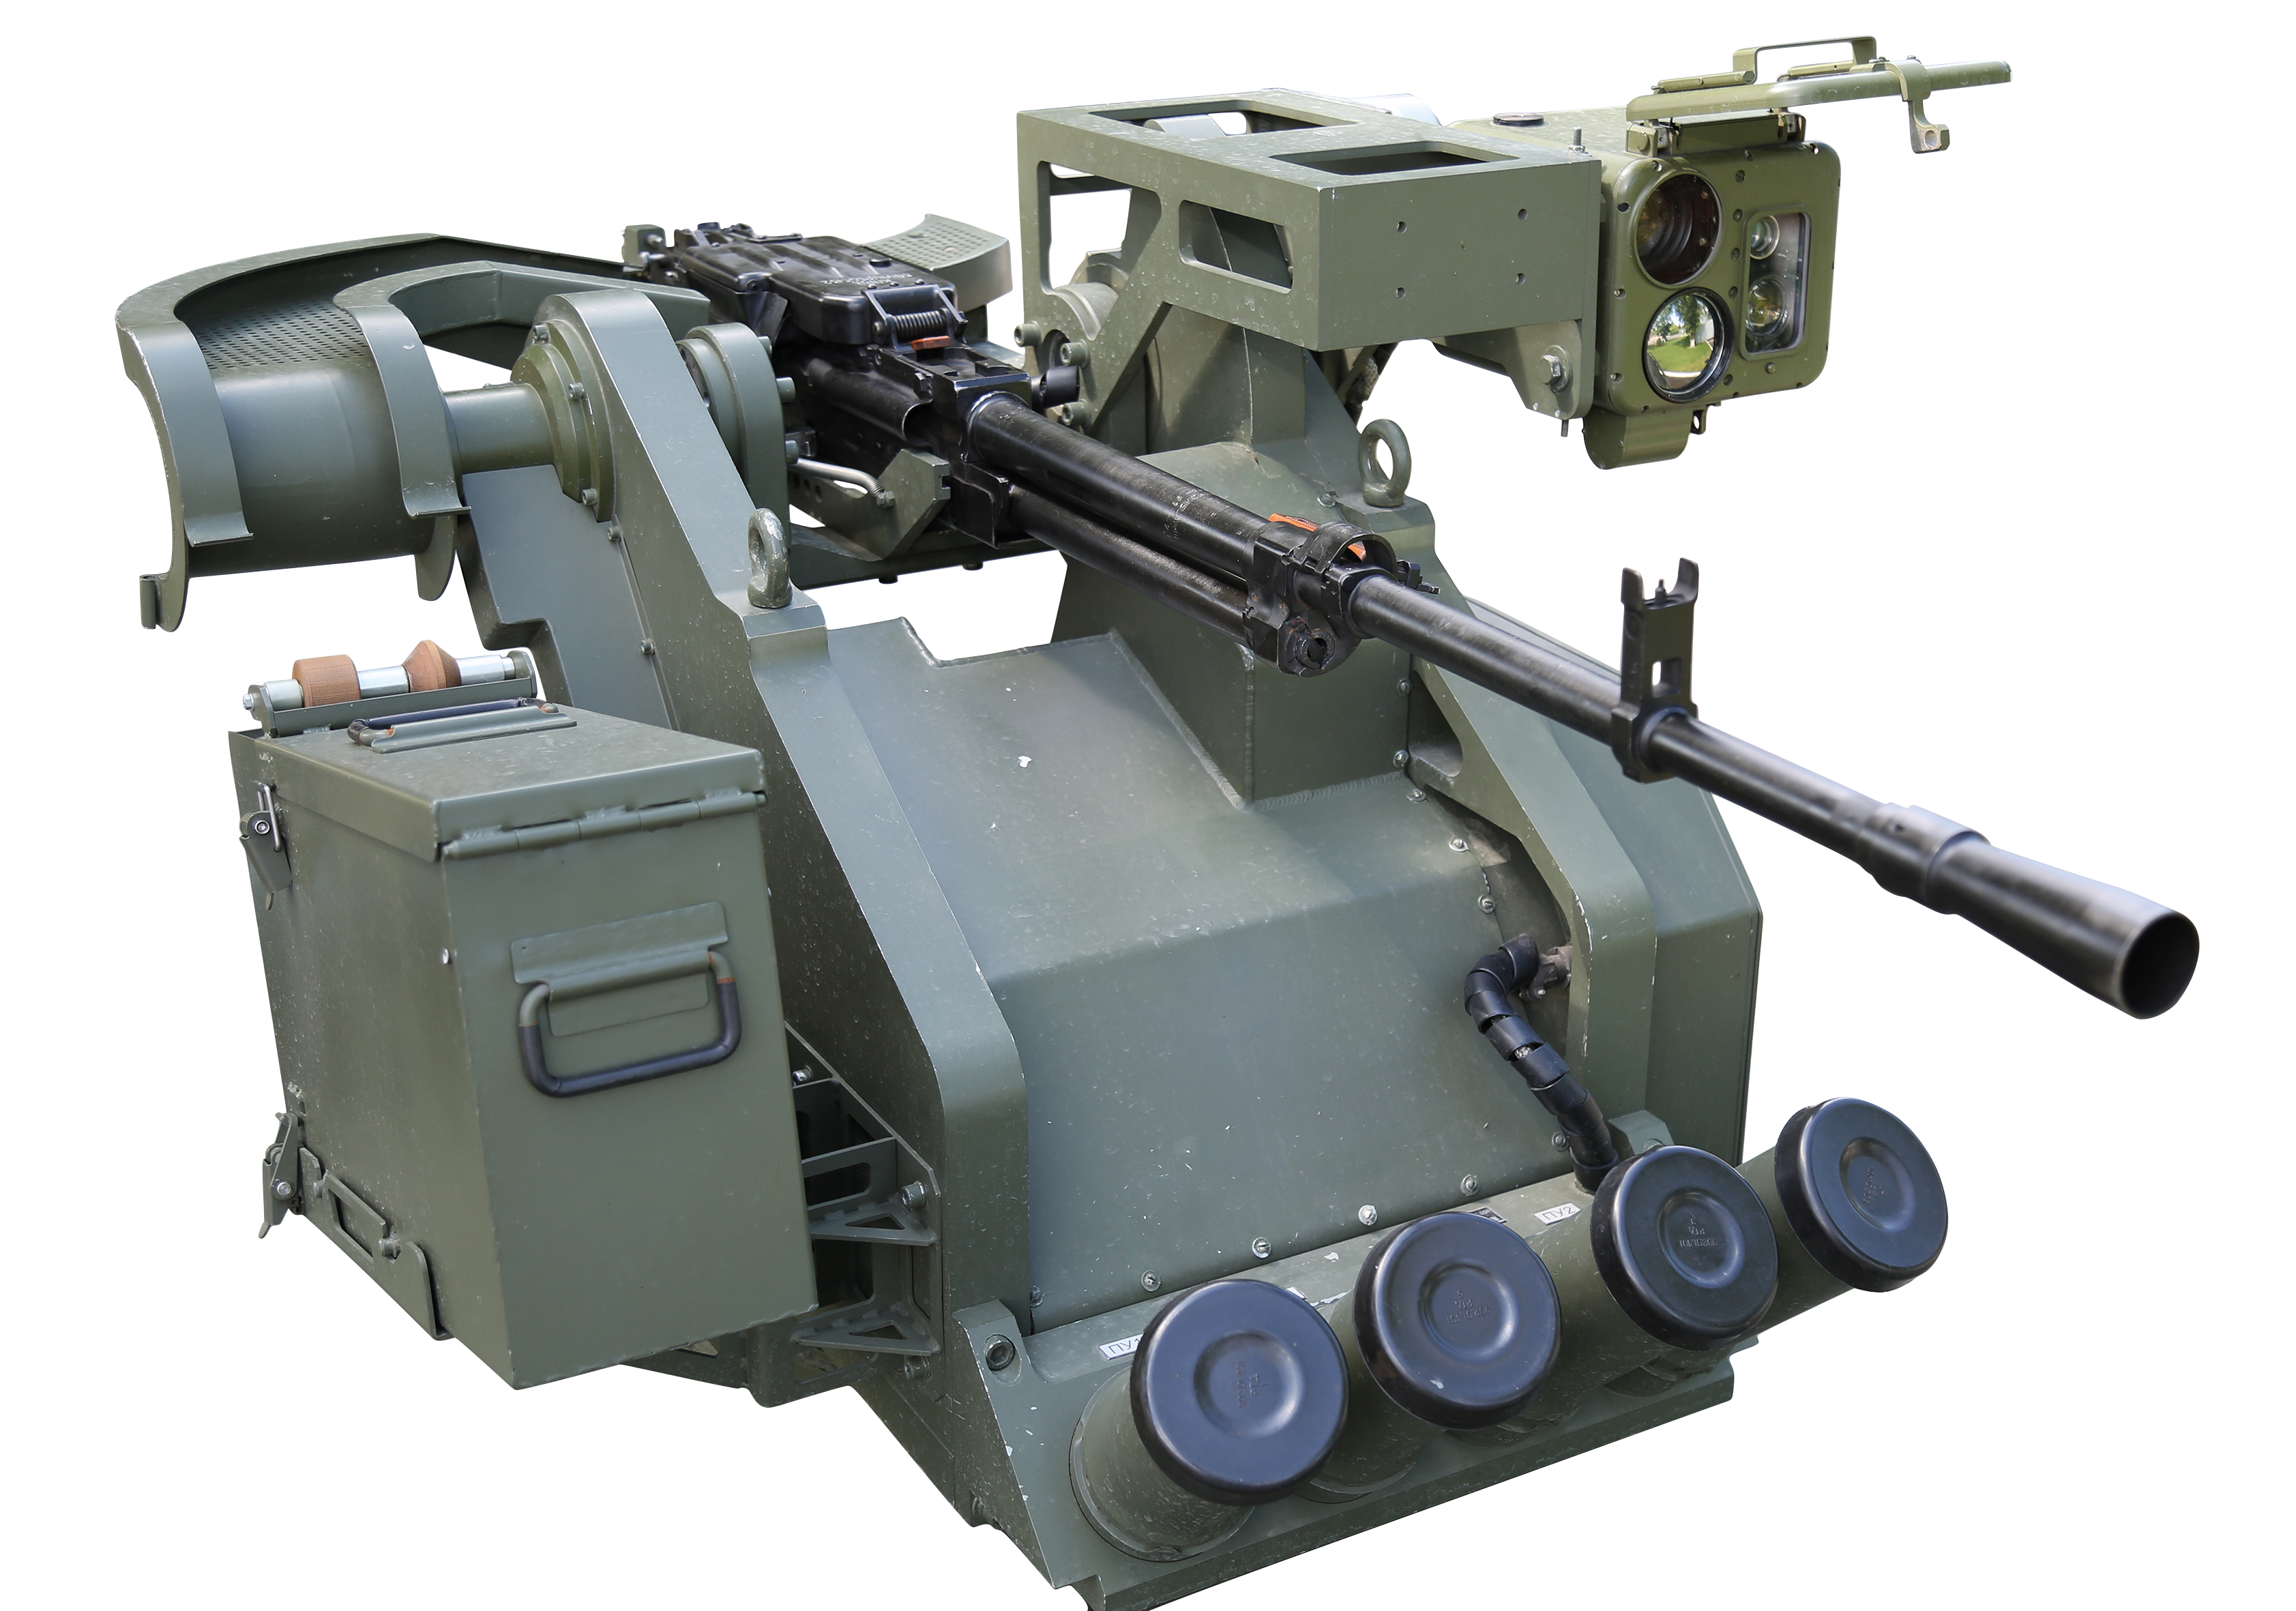
\includegraphics[width=1\linewidth]{irod_arbalet}
	\caption{Az orosz Arbalet-DM rendszer}
	\label{fig:irod_arbalet}
\end{figure}


\begin{figure}[h!]
	\centering
	\includegraphics[width=1\linewidth]{irod_defnder}
	\caption{A belga DeFNder rendszer}
	\label{fig:irod_defnder}
\end{figure}
\end{document}